\documentclass{aa}  
\usepackage{rotating}
\usepackage{natbib}
\usepackage{amsmath}
\bibpunct{(}{)}{;}{a}{}{,} % to follow the A&A style

\newcommand{\kms}{km s$^{-1}$}
\newcommand{\bpb}{Beta Pictoris b}
\newcommand{\bp}{Beta Pictoris}

\usepackage{color}
\usepackage{hyperref}
\hypersetup{colorlinks=true,allcolors=[rgb]{0,0,0.8}}

\usepackage[nolist,nohyperlinks]{acronym}
\newacro{harps}[HARPS]{High Accuracy Radial Velocity Planet Searcher}
\newacro{uves}[UVES]{Ultra-violet Visible Echelle Spectrograph}
\newacro{feb}[FEBs]{Falling Evaporating Bodies}

%
\usepackage{graphicx}
%%%%%%%%%%%%%%%%%%%%%%%%%%%%%%%%%%%%%%%%
\usepackage{txfonts}
%%%%%%%%%%%%%%%%%%%%%%%%%%%%%%%%%%%%%%%%
%\usepackage[options]{hyperref}
% To add links in your PDF file, use the package "hyperref"
% with options according to your LaTeX or PDFLaTeX drivers.
%
\usepackage{showyourwork}

% text highlighting
\usepackage{soul}
\sethlcolor{yellow}

\usepackage[version=4]{mhchem}
% the three lines suppress the hyperref 'link empty' warnings
% explanation at: https://tex.stackexchange.com/questions/345764/journal-class-shows-package-hyperref-warning-suppressing-link-with-empty-targe
\makeatletter
\renewcommand*\aa@pageof{, page \thepage{} of \pageref*{LastPage}}
\makeatother

\begin{document} 


   \title{Upper Limits on CN from Falling Evaporating Bodies\\seen towards \bp{}}

   \author{M.A. Kenworthy
          \inst{1}
          \and
          E. de Mooij\inst{2}
          \and
          C. Opitom\inst{3}
          \and
          A.\ Brandeker\inst{4}
          \and 
          F. Kiefer\inst{5}
          \and
          A. Fitzsimmons \inst{1}
          }

   \institute{Leiden Observatory, Leiden University, P.O. Box 9513, 2300 RA Leiden, The Netherlands\\
              \email{kenworthy@strw.leidenuniv.nl}
         \and
             Astrophysics Research Centre, School of Mathematics and Physics, Queen’s University Belfast, BT7 1NN Belfast, UK
        \and
             Institute for Astronomy, University of Edinburgh, Royal Observatory, Edinburgh EH9 3HJ, UK
        \and
        Institutionen f\"{o}r astronomi, Stockholms universitet, AlbaNova universitetscentrum, 106 91, Stockholm, Sweden
        \and
        LESIA, Observatoire de Paris, Université PSL, CNRS, 5 Place Jules Janssen, 92190 Meudon, France}

   \date{Received XXXX; Accepted XXXX}

% \abstract{}{}{}{}{} 
% 5 {} token are mandatory
 
  \abstract
  % context heading (optional)
  % {} leave it empty if necessary  
   {Beta Pic has \ac{feb} which are seen as variable transient absorption features towards \bp{}.}
  % aims heading (mandatory)
   {To detect cyanogen (\ce{CN}) in the \ac{feb} spectrum, confirming that they are similar to comets in the Solar System.}
  % methods heading (mandatory)
   {We combine the \ac{harps} spectra from the past 20 years to make a high signal to noise ratio spectrum and look for the \ce{CN} band head. We also combine \ac{uves} data to confirm our non-detections/detections.}
  % results heading (mandatory)
   {No \ce{CN} is seen to a level of XXX ppt, indicating that there is less \ce{CN} in these \ac{feb} than Solar system comets.}
  % conclusions heading (optional), leave it empty if necessary 
   {\ac{feb} are not Solar System comets in composition.}

   \keywords{comets --- transits, spectroscopy}

   \maketitle
%
%________________________________________________________________

\section{Introduction}

The formation and evolution of planets and their attendant moons is thought to occur in the first few ten million years of the stellar system \hl{REF}.
%
Comets deliver volatiles across menay different distances within the Solar system, from the outermost reaches of the Oort cloud in to the terrestrial planets.
%
It is therefore important to understand the distribution, nature and chemical composition of exocomets in other planet forming systems.

One of the closest young systems is Beta Pictoris, which has been studied intensively both with direct imaging and with spectroscopy.

Beta Pictoris is a young, early type star whose stellar chromosphreic lines show rotational broadening of 200 km/s \hl{REF}.
%
The Ca H and K lines show deep absorption to 0.1 of the continuum level.
%
A consistent and stable narrow absorption feature with a FWHM of a few km/s is explained by the presence of the circumstellar material.
%
There exist transient, irregular shaped absorption features in the spectra of the star.
%
These appear and disappear on hour long timescales, and show a different range of morphologies, predominantly seen at bluer wavelengths. \hl{[REF]}.
%
Intensive spectroscopic monitoring over several hours show changes of radial velocity of these components consistent with elliptical orbits.
%
The absorption is hypothesised to be due to the evaporation of infalling bodies that pass within a few stellar radii of the star, resulting in sublimation of material that produce a large coma containing the Calcium atoms which are then seen as an additional absorption component \hl{[REF REF]}.

From the multiple detections of exocomets in spectroscopy towards Beta Pictoris, the broadband detection of exocomet tails transiting a star were seen initially detected towards the star KIC~3542116 \citep{Rappaport18} with the {\it Kepler} satellite \hl{REF} and subsequently detected in TESS data towards Beta Pictoris \citep{Zieba19}.
%
Observations of Beta Pictoris in subsequent TESS sector revealed over two dozen transits whose depth follows a power law distribution similar to those of the Solar system \citep{LecavelierdesEtangs22,Pavlenko22}.



%Short Beta pic description, previous detection of species in optical (CaII, NaI, FeI).


To the contrary of what is observed in the case of \ac{feb}, most molecular and atomic signatures detected in the coma of Solar system comets are emission lines/bands instead of absorptions.

Spectroscopic observations of Solar system comets when they are very close to the Sun are rare due to observational difficulties.
%
%The only comet spectroscopically observed closer than 0.2~au from the Sun is C/1965~S1 Ikeya-Seki.
%
%For this comet, it was noticed that the main emission bands/lines detected in its optical spectrum dramatically changed while the comet approached the Sun.
%
%At distances greater than 0.4~au, \ce{CH}, \ce{CN}, \ce{C2}, and \ce{C3} emission bands dominated the spectrum, but at 0.15 au from the Sun, the only molecular emission detected was \ce{CN}, while numerous atomic lines were visible \citep[\ce{[\ion{O}{i}], \ion{Na}{i}, \ion{K}{i}, \ion{Ca}{ii}, \ion{Cr}{i}, \ion{Mn}{i}, \ion{Fe}{i}, \ion{Ni}{i}, \ion{Cu}{i}, \ion{V}{i}; ][]{Dufay65,Thackeray1966,Preston1967,Slaughter1969}.
%%\ion{Ca}{ii} and \ion{Fe}{i} have only been spectroscopically observed via emission lines in the sun-grazing comet C/1965~S1 Ikeya-Seki.
%
For this comet, it was noticed that the main emission bands/lines detected in its optical spectrum dramatically changed while the comets approached the Sun.
%
At distances greater than 0.4~au, \ce{CH}, \ce{CN}, \ce{C2}, and \ce{C3} emission bands dominated the spectrum.
%
However, at 0.15~au from the Sun, the only molecular emission detected was \ce{CN}, while numerous atomic lines were visible \citep[\ion{[O]}{i}, \ion{Na}{i}, \ion{K}{i}, \ion{Ca}{ii}, \ion{Cr}{i}, \ion{Mn}{i}, \ion{Fe}{i}, \ion{Ni}{i}, \ion{Cu}{i}, \ion{V}{i}; ][]{Dufay65,Thackeray1966,Preston1967,Slaughter1969}.
%
Additionally, a tail of \ion{Fe}{i} atoms was proposed to explain a linear feature imaged in the tail of sungrazing comet C/2016~P1 McNaught 2006P1 \citep{Fulle2007}. 

On the other hand, \ion{Na}{i} D-line emission has been observed in many comets within $r \sim 1$ au of the Sun, where either the emission was much brighter than the foreground sky emission, or the comet was observed at high spectral resolution enabling separation from the telluric lines \hl{REFs}.
%
The high efficiency of the \ion{Na}{i} D transition makes it easily detectable, even for relatively low column density.
%
A notable discovery was a spectacular tail of \ion{Na}{i} associated with comet C/1995 O1 Hale-Bopp at $r\sim 1$ au, formed by radiation pressure on the neutral atoms before ionisation \citep{Cremonese1997}. 

These characteristics imply that \ion{Ca}{ii} and \ion{Fe}{i} are predominantly locked up within cometary dust gains, and only observed when a comet is close enough to the Sun to allow their sublimation.
%
This occurs at $r\leq 0.03-0.06$ au for a dust grain with Bond albedo $\sim0.01$ and a sublimation temperature of $T\simeq 1600$K, depending on the thermal model assumed.
%
On the other hand, the origin of the \ion{Na}{i} tail observed in numerous comets at larger distances from the Sun is still not very well understood \citep{Cremonese02}.
%
Release from dust grains as well as molecular processes have been suggested as possible sources of \ion{Na}{i} in the coma and tail of comets annd explain its presence at large solar distances \citep{Cremonese1997}.
%Na appears to be weakly bound to the dust grains and released at larger solar distances.

For the majority of Solar system comets, their optical spectra are dominated by the reflected sunlight from dust grains in their comae, plus molecular and atomic emission lines \citep[e.g. ][]{hyland2019}.
%
Most of the neutral and ionic molecular emission results from resonance fluorescence with solar photons. Some species, such as \ce{H2O+} and \ce{CO+} result from ionization of parent molecules (i.e. molecules released directly by the sublimation of nuclear ices), all other molecules observed are second generation species, often created via photodissociation of parent molecules or released by organic-rich grains in the coma.
%
Another process also observed in optical spectrum of comets is prompt atomic emission  ([\ion{O}{i}], [\ion{C}{i}], and [\ion{N}{i}]).
%
Those forbidden transitions are the result of atoms produced in an excited state by the photodissociation of parent molecules in the coma. 

Of all cometary gas emission, the highest signal to noise normally occurs with the \ce{CN} (0-0) band at $\lambda\simeq 3880$\AA.
%
It is usually the first emission detected in the optical spectrum of a comet as it approaches the Sun, and as been detected in the coma of comets observed at relatively large distances from the Sun \citep[e.g. ][]{Fitzsimmons1996}.
%
The relative abundance in the coma of most comets of \ce{CN/OH}$\simeq500$ \citep{AHearn1995}, together with its high fluorescence scattering efficiency factor of $\sim$ 2.6 photons/sec/molecule at 1~au from the Sun and $\dot{r}\simeq 0$ \citep{Schleicher2010}, gives rise to a clear signature of a cometary gas comae.
%
Historically, the \ce{CN} was believed to be created from photodissociation of \ce{HCN}, which is present in abundances of the order of 1\% relative to water in cometary ices.
%
High-spatial resolution sub-mm mapping of \ce{HCN} distributions supports a nuclear source in some comets \citep{Cordiner2014}.
%
However, it is now known that in many comets a substantial fraction of \ce{CN} is released from sub-micron dust grains in the inner coma of comets \citep[e.g. ][]{Fray2005}. 

The \ce{C2} (0-0) band at $\lambda\simeq 5160$\AA \ may be of comparable flux, but has a lower contrast with the underlying dust grain continuum due to its wider bandwidth.
%
The \ce{OH} (0-0) band at $\lambda\simeq 3080$ \AA \ generally has higher flux, but unless observed from space the high terrestrial atmospheric absorption severely diminishes the observed flux.
%
Strong \ce{CO+} emission bands have also been observed in a number of comets (the strongest ones are the (3-0) and (2-0) $\mathrm{A^2\Pi-X^2\Sigma}$) \hl{REFS}).
%
However this is normally significantly weaker than the observed \ce{CN} emission, with only \hl{number of comets} comets.

Given the ubiquitous signature of \ce{CN} emission in Solar system comets, we have embarked on an archival search for this species in the \ac{feb} around \bp{}.
%
Detection of this species would provide a solid link between cometary bodies in our Solar system and the \bp{} system.

We detail the observations in Section~\ref{sec:data}, along with the correction for the echelle blaze function and normalization of the spectra to a continuum.
%
Our search for \ce{CN} relies on a cross correlation search with a theoretical absorption spectrum for the molecule in Section~\ref{sect:CNsearch}, and the discussion and interpretaion is in Section~\ref{sec:discuss} with our conclusions in Section~\ref{sec:conclusion}.

\section{Data description and analysis}\label{sec:data}

For the study in this paper, we use all the publicly available data from the \ac{harps} and the ESO 3.6m telescope in Chile.
%
In addition, we complement this with observations with the \ac{uves} at the Very Large Telescope in Chile. 

\subsection{HARPS observations}

We collated all publicly available HARPS observations of \bp{} obtained between October 2003 and \hl{March 2020}.
%
Although these observations cover a large baseline, the time between visits varies between 1 day and $\sim$2.2 years.
%
Similarly, the number of observations per epoch spans a wide range, between \hl{1 and 356} exposures, while the exposure times vary between \hl{12 and 900} seconds. This results in a SNR range per exposure between \hl{NNNN and MMMM}, and a nightly SNR between \hl{NNNN and MMMM}.
%
To avoid potential edge effects from order merging,  we used the E2DS files downloaded directly from the ESO archive for our analysis.

% \hl{Q: Do we want to put an observing log in the appendix?}
% \hl{Q: Do we want to attempt to use the S1D, as they may have less issues with wiggles if the blaze profile was removed.}



\subsection{UVES observations}

To supplement the HARPS observations, we use 160 epochs of \ac{uves} observations obtained between 01 April, 2017 and April 18, 2018 under programme 599.C-0751.
%
The details for these observations are given in \cite{vansluijs2019}, and summarised here.
%
These observations were all obtained using the same instrument setup.
%
We used the standard 437+760 mode of \ac{uves}, which uses the \#2 dichroic to allow simultaneous observations in both the red and blue arm.
%
In this mode, the CD\#2 and CD\#4 cross-dispersers are used in the blue and red-arm, respectively, providing a simultaneous wavelength coverage of $\sim 3730$ \AA{} to $\sim 5000$ \AA{} in the blue arm, and $\sim 5650$ \AA{} to $\sim 9560$ \AA{} in the red arm.
%
For the remainder of the paper, we will only focus on the data from the blue arm of \ac{uves}, as this covers the strong \ce{CN} (0-0) band-head seen in Solar system comets.
%
For the blue arm, a 0.3''-wide slit was used to obtain the highest possible resolving power ($\sim$90,000 before an intervention on the instrument in October 2017, and $\sim$100,000 after the intervention). 

The data were reduced using the ESO \ac{uves} pipeline version \hl{6.1.6} through ESO Reflex tool in order to provide as homogeneous a dataset as possible. The flat-field was applied on a pixel-by-pixel basis. \hl{The pipeline was set to output the intermediate products and the blaze-corrected spectra before merging were used for our analysis, as the order-merging could introduce systematics in the overlap region. Optimal extraction was performed, using an empirical profile}

\subsection{Initial data processing}
Starting from the 2d spectra, the data from both instruments was processed in similar ways.
%
Each order was treated separately, with the main focus on orders \hl{4 and 8} for HARPS and \hl{4, and 7} for UVES as those orders contain the main \ce{CN} bandhead as well as the \ion{Ca}{ii} H line, which are used to identify the exocomets.
%
All the spectra were transformed into the stellar rest-frame and onto a common wavelength grid using linear interpolation. For UVES, the \ce{Fe} \hl{NNNN angstrom} line was used to track global wavelength drifts between different exposures which were corrected for at the same time. To measure these, a Gaussian was fit to the line, and the velocity offset from the rest frame position determined. 

%
After all the spectra were all transformed into the stellar rest frame, an average nightly spectrum was made from all spectra within a night for each of the nights of observations. This was done after correcting for variations in the effective blaze profile (e.g., due to instrumental changes, differential slit/fiber losses, atmospheric absorption etc.), as outlined below. Note that after this correction, the HARPS data still have the overall instrumental blaze-profile, while the 2d-spectra from UVES were already corrected for this.


\subsection{Effective Blaze function correction}\label{sect:blaze}

One of the nights with a high signal to noise was chosen to act as an initial estimate for the blaze function (the night of \hl{DATE} for HARPS and \hl{DATE} for UVES). The individual spectra in this night were averaged together to further boost the signal-to-noise ratio. Subsequently, each individual spectrum was divided by this reference spectrum to highlight the changes in the effective profile. This ratio spectrum was subsequently binned using a bin-width of \hl{101} pixels using a robust algorithm to remove outliers within each bin. This binned ratio was than fit using a \hl{second} order polynomial. The original spectrum was finally divided by this polynomial to correct for the changes.

Note that for HARPS, the change of fiber in June 2015 (JD$\sim$2,457,180) resulted in an overall change of the blaze profile, and therefore, the spectra before and after this date were separately post-processed as outlined below in the Sect.~/ref{sect:starcor}.



\subsection{Combining the spectra and flattening them}\label{sect:comb}
After the blaze-variation corrections, all the spectra within a night are combined in order to further boost the signal-to-noise and improve the detection limits. Each individual spectrum was weighted using the average signal-to-noise ratio provided in the header for orders \hl{NN and MM, and OO and PP} for HARPS and UVES respectively.

%For the spectra within a given night:
%
%\begin{itemize}
%\item We median combine all the nights together.%
%
%\item Bin the spectrum and clip it, interpolate using a cubic spline.
%
%\item Divide this interpolated cubic spline into each of the nightly spectra.
%
%\end{itemize}

\subsection{Removing the stellar spectrum}\label{sect:starcor}
The processing up to this stage removes most of the variations in the effective blaze function, but the overall stellar spectrum and, for HARPS, shape of the blaze profile, are still present and need to be removed. 

For both HARPS and UVES we first perform a second iteration of blaze corrections using a  stellar spectrum constructed by averaging the spectra from periods with a low comet activity (see \hl{Sect.}~\ref{sect:FEBident}. For HARPS this is done separately pre- and post-fiber change. The correction is done similar to Sect.~\ref{sect:blaze}, however for both UVES and HARPS a \hl{4th order} polynomial was used.

After this post-processing the overall (residual) blaze profile and stellar spectrum still need to be removed. Care must be taken to prevent the removal of (potential) narrow features from the circumstellar disk (as seen in e.g., the \ce{Fe} and \ion{Ca}{II} lines). This is done by combining the nightly spectra without significant cometary activity (see Sect.~\ref{sect:FEBid}) and binning this stacked spectrum in wavelength in bins of 21 pixels. Before binning, the spectrum in each bin was MAD (median absolute deviation) clipped to within $\pm$4.5 MAD of the median of the flux in the bin. The clipped average of the fluxes within each bin was used. Subsequently, the overall spectrum of the star and (residual) blaze was determined by cubic interpolation across the binned points, and divided out of the spectrum for each night. As before, for HARPS this was done separately pre- and post-fiber change.




%Subsequently, we applied a correction for variations in the instrumental blaze by selecting a reference spectrum and dividing all the spectra by this reference. The ratio was then binned, removing outliers, and a polynomial was fit to the data.
%
%For \ac{uves} we used a Nth degree polynomial, while for \ac{harps} we used a 2nd degree polynomial.
%
%This polynomial was then divided from the spectrum under consideration. We note that the blaze correction will also remove non-instrumental effects, including variations in atmospheric transmission and seeing.

%The blaze-corrected spectra taken within a night were averaged together [Should we use a weighted average?].
%
%We note that for \ac{harps}, the 2d-unmerged spectra still contain the overal instrumental blaze-profile, which is (partially) corrected for by using a dedicated blaze-frame obtained from the archive, which removes most, but not all, of this profile. 

\section{Searches for \ce{CN}}\label{sect:CNsearch}

After the initial data analysis, we proceed to with our search for lines from \ce{CN}.
%
Although we are interested in lines from the exocomets, we first co-add the data from all the individual epochs, in the stellar rest-frame, to obtain a deep search for circumstellar \ce{CN} absorption.
%
\hl{These coadded spectra for }\ac{harps} and \ac{uves} are shown in \hl{Figure}.
%
No obvious feature from the \ce{CN} band jumps out, and we need to combine the signal from the lines within the \ce{CN} band to improve the detection limits.

Since the exocomets have a clear radial velocity with respect to \bp{}, and since each exocomet will have its own distinct velocity, we selected the \hl{NN} epochs with the strongest exocometary features, a seen in the \ion{Ca}{ii} H line. 

\hl{TODO FIGURE: Just spectrum coadded} in stellar rest frame same for comet rest frame in the \ce{CN} band wavelength range, with the \ce{CN} band overplotted.

\subsection{Identifying exocomets from \ion{Ca}{ii} H line}\label{sect:FEBid}
The comet features in the \ion{Ca}{ii} H-line ($\lambda=3968. \AA$) were identified after removing the overall stellar line-profile and avoiding the absorption from the circumstellar disk by excluding the central \hl{NN} km\,s$^{-1}$.
%
The deepest absorption feature in each observing night was selected, and the location and depth stored.
%
For the comet sample we selected features deeper than \hl{60\% and 40\%} for HARPS and UVES, respectively, while spectra with features below 15\% for both HARPS and UVES were flagged as `low activity'.
%
An example of the \ion{Ca}{ii} H line for a night with a strong comet and for a night with a weak comet are shown in Figure \hl{XXXX}.
%
The distribution of feature location and depth is shown in \hl{Figure}.

plotFEbs for the above first two figures!

The spectra for the strong comet sample were coadded, and the combined spectrum for the HARPS data is shown in \hl{Figure}.
%
As with the circumstellar \ce{CN}, there are no obvious lines from \ce{CN} visible, and we will need to combine multiple lines to improve the signal-to-noise ratio, and see if there is any \ce{CN} present. 
%
%The spectra with only weak exocometary features were co-averaged in the stellar rest frame in order to create a stellar master spectrum. This master-spectrum was divided out of all the remaining spectra in order to create relative spectra. 
%
%The relative velocities of the exocomets were determined by ......., and the spectra were shifted to the rest-frames of these comments, before being combined.
%
%The combined exocomet aligned spectra for both the \ce{Ca} H\&K lines and \ce{CN} band are shown in Fig.~\ref{fig:coadd_exocomets}. As can be seen no signal is visibly present.
%

\begin{figure}
    \begin{centering}
        \includegraphics[width=\columnwidth]{figures/CN_ACF.pdf}
        \caption{\ce{CN} autocorrelation function for different temperatures.}
        \label{fig:CN_ACF}
        \script{plot_CN_ACF.py}
    \end{centering}
\end{figure}

\subsection{Cross-correlation with \ce{CN} models}\label{sect:CCF}


\begin{figure}
    \begin{centering}
        \includegraphics[width=\columnwidth]{figures/two_CN_temps.pdf}
        \caption{Model absorption spectrum for \ce{CN} at two temperatures.}
        \label{fig:CN_theory}
        \script{plot_two_CN_temps.py}
    \end{centering}
\end{figure}


To combine the signal from the many \ce{CN} lines, we cross-correlate the data for each night with a grid of model of \ce{CN}.
%
Cross-sections for \ce{CN} were obtained from ExoMol \hl{REFERENCES HERE} and the cross-sections were calculated using \hl{NEED SOME DETAILS...}. 
%
We made models for a wide range of temperatures (T$=$\{10, 20, 30, 50, 100, 200, 300, 500, 1000, 2000, 3000\} K) and column densities\footnote{Note that technically, for optically thin lines, this assumes a filling factor $f=1$.
%
Since $f$ is unknown, we actually measure N$f$} (N=\{$10^{11} \ldots 10^{15}$\} cm$^{-2}$.
%
Each of the models was then convolved to include an effective velocity dispersion using a Gaussian for FWHM=\{2.9, 5, 10, 15, 20\} km\,s$^{-1}$.
%
A value of 2.9 km\,s$^{-1}$ corresponds approximately to the instrumental resolution of HARPS.
%
The theoretical spectra of \ce{CN} for several different temperatures are shown in Figure~\ref{fig:CN_theory}.

Even after cross-correlating, the stacked CCFs (see Fig.~\ref{fig:ccf} do not show any clear signals, and we therefore proceed to estimate our detection limits.

\begin{figure}
    \begin{centering}
        \includegraphics[width=\columnwidth]{figures/FEB_velocity_depth.pdf}
        \caption{Peaks and radial velocities of exocomets identified in the stellar spectrum.
        %
        The peaks are normalised such that 1 represents total absorption in the spectrum.
        %
        Peaks closer than 10 km/s are masked out due to contamination from the circumstellar material.
        %
        Peak values above 0.6 are counted as exocomets and those below 0.15 as stellar only.}
        \label{fig:FEB_velocity}
        \script{plot_FEB_velocity_depth.py}
    \end{centering}
\end{figure}


\begin{figure}
    \begin{centering}
        \includegraphics[width=\columnwidth]{figures/ccf_mean.pdf}
        \caption{Cross correlation for different number densities of \ce{CN} averaged over many spectra.}
        \label{fig:ccf_mean}
        \script{plot_ccf_mean.py}
    \end{centering}
\end{figure}

\begin{figure}
    \begin{centering}
        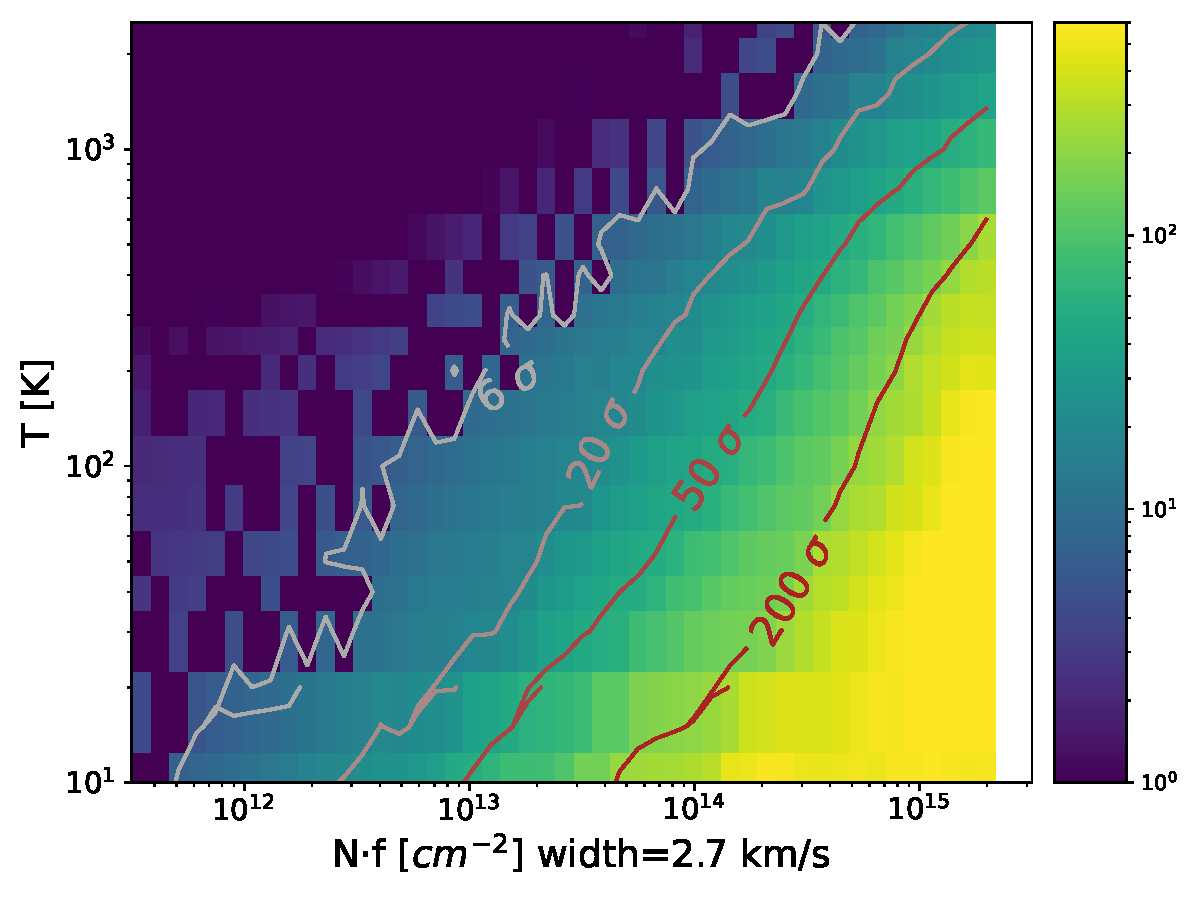
\includegraphics[width=\columnwidth]{figures/HARPS_CN_stellar_frame.pdf}
        \caption{\ce{CN} measurement limits in the stellar rest frame for a \ce{CN} line width of 2.7\kms{}. Contours show signal to noise upper limits.}
        \label{fig:CN_stellar_frame}
        \script{plot_HARPS_CN_stellar_frame.py}
    \end{centering}
\end{figure}


\begin{figure}
    \begin{centering}
        
\includegraphics[width=\columnwidth]{figures/asdf.png}
        \caption{Test picture}
        \label{fig:test}
    \end{centering}
\end{figure}


\begin{figure*}
    \begin{centering}
        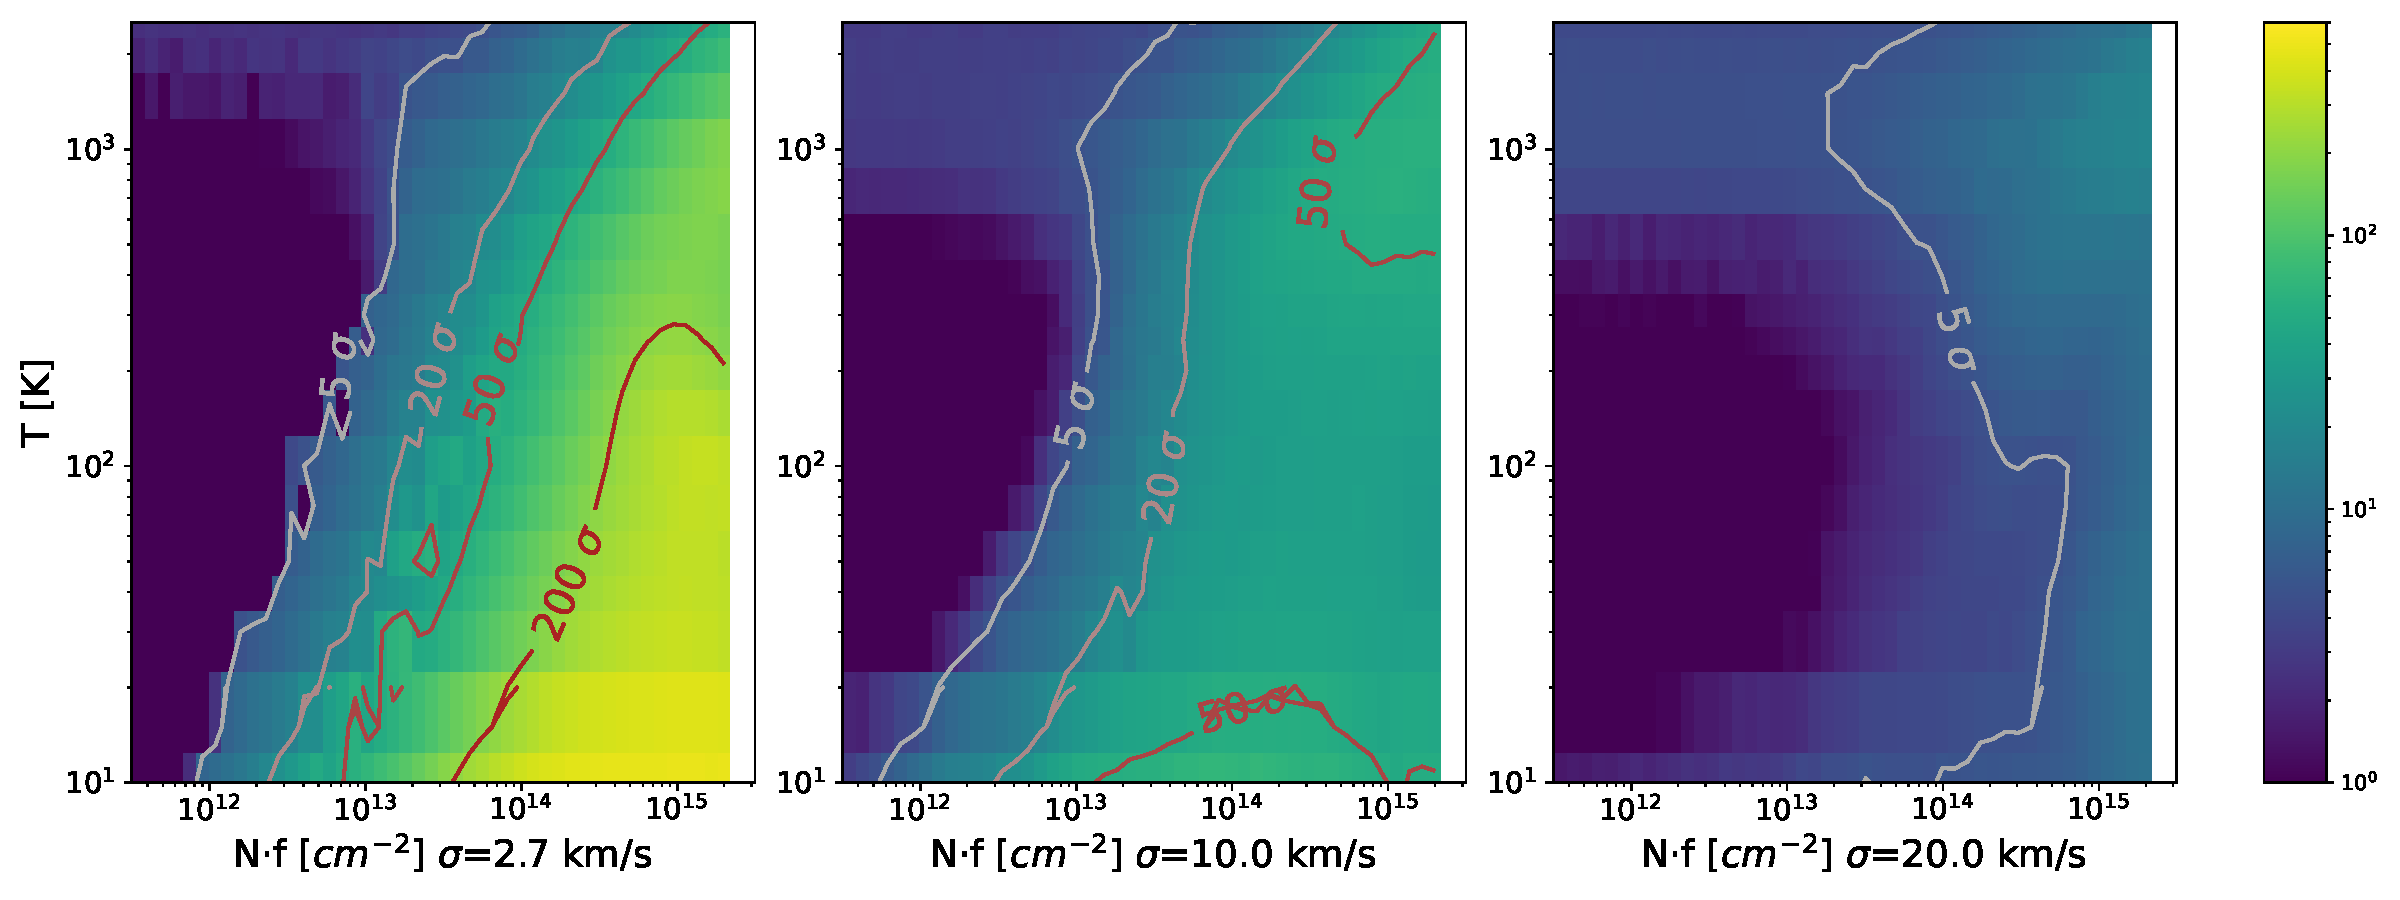
\includegraphics[width=\linewidth]{figures/HARPS_CN_exocomet_frame.pdf}
        \caption{\ce{CN} measurement limits in the exocomet frame for a \ce{CN} line width of 2.7, 10 and 20\kms{}. Contours show signal to noise upper limits.}
        \label{fig:CN_exocomet_frame}
        \script{plot_HARPS_CN_exocomet_frame.py}
    \end{centering}
\end{figure*}




% \begin{figure}
%     \begin{centering}
%         
\includegraphics[width=\columnwidth]{figures/asdf.png}
%         \caption{Test picture}
%         \label{fig:test}
%     \end{centering}
% \end{figure}


% \begin{figure}
%     \begin{centering}
%         \includegraphics[width=\columnwidth]{figures/HARPS_CN_grid.pdf}
%         \caption{Confidence intervals for the signal to noise of \ce{CN} spectra using \ac{harps} spectra of \bp{}.}
%         \label{fig:HARPS_CN_grid}
%         \script{plot_HARPS_CN_grid.py}
%     \end{centering}
% \end{figure}

%\subsection{Other Species? CO$^+$, C$_2$?}

\subsection{Estimating the \ce{CN} column density limits}\label{sect:CNlim}

To estimate the limits on the \ce{CN} detection, we perform injection and recovery tests.
%
We injected models for different temperatures, column densities and velocity broadening into the nightly stacked spectra (Sect.~\ref{sect:comb}, and then processed them in the same way as the original data (i.e., correct for residual blaze variations, removal of the stellar envelope and cross-correlation).
%
This was done for all spectra with the injected signal in the stellar rest frame as well as for the sample of spectra with strong cometary activity in the rest frame of the strongest exocometary feature per night.

The individual CCFs show some overall slopes and offsets, and we fit each individual CCF with a combination of a second-order polynomial baseline and a Gaussian with the position fixed to 0 \kms{} in its rest frame.
%
The fit has five free parameters: the amplitude of the peak, the width of the peak, and the offset, slope, and intercept of the baseline.
%
To avoid the aliasing peaks of the \ce{CN} band (see Figure~\ref{fig:CN_theory}), we only fit the central $\pm$35 \kms{} of the CCF.
%
Fitting is done using the curve\_fit function from SciPy \citep{2020SciPy-NMeth}.
%
We correct each of the individual CCFs for the baseline and then stack the corrected CCFs to obtain our master CCF that we use for determining the upper limit.
%
The noise on each point in the master CCF is determined by taking the standard deviation in time for each pixel and dividing that by the square root of the number of points.

This master CCF is then fitted in the same way as the nightly CCFs, and the uncertainties on the parameters is taken directly from {\tt curve\_fit} assuming no covariance between the parameters.
%
The final detection significance for the injected models is determined by the amplitude divided by its uncertainty, and shown in Figure~\ref{fig:CN_stellar_frame} for the circumstellar gas and in Figure~\ref{fig:CN_exocomet_frame} for the strongest exocomet features.

\section{Discussion}\label{sec:discuss}

%\subsection{Summary of \ce{CN} in comets}

\ce{CN} is one of the brightest optically active species in cometary comae.
%
It is a minor component of the gas coma, with a production rate by number $\sim 1/500$th that of water. 

Most studies of Solar system comets simply observe the \ce{CN} molecules via optical fluorescence.
%
From measurements and simple physical arguments the \ce{CN} absorption/emission is optically thin everywhere.
%
This means a flux from part of the coma can immediately be converted to a column density using a photon scattering efficiency for the molecular band.

\ce{CN} in solar system comets comes from two sources.
%
Sublimation of nucleus near-surface ices releases \ce{HCN}, which then photo-dissociates into \ce{CN}.
%
This in turn eventually photo-dissociates into the component atoms.

$$\ce{HCN} +\gamma \rightarrow \ce{H}+\ce{CN}$$
$$\ce{CN} + \gamma \rightarrow \ce{C}+\ce{N}$$

Since Halley in 1986, it has also been known that dust grains ejected from the nucleus also directly release \ce{CN} into the coma.
%
However, \ce{CN} production in comets is usually dominated by nuclear ice sublimation.

The resulting \ce{CN} coma will have a true space density and apparent column density distribution centrally peaked at the comet nucleus.
%
For Solar system comets, column densities are often converted to an overall production rate $Q_{\ce{CN}}$ molecules/sec via an analytical model known as the ``Haser'' model.
%
For this model there are only 3 parameters; the effective destruction scale length $l_p$ of the parents of \ce{CN} (\ce{HCN}+dust), the photodissociation scale length $l_{\ce{CN}}$ of \ce{CN}, and the gas outflow velocity $v$.
%
The Haser model is somewhat simplistic but it represents the data well.

\subsection{Example comet - 1P/Halley}

We take the observed activity of 1P/Halley in 1985/86 as an example for our estimates.
%
Although most comets we observe are far less active than Halley, there are quite a few comets with activity similar to it.
%
Given that we will be dominated by the most active comets at \bp{}, this seems reasonable as something that can be later scaled to the brightest comets such as Hale-Bopp.
%
When Halley was at $\sim 1$ au from the Sun, it was measured to have $Q_{\ce{CN}}\simeq 10^{27}$ molecules/sec using Haser models.
%
The assumed outflow velocity in the models was generally  $0.85 - 1$ \kms{} at this distance.

For solar system comets, the normal Haser scale lengths used \citep{Cochran86,AHearn1995} are:

$$lp=1.7\times10^4r_h^2\:{\rm km}$$

$$l_{\ce{CN}}=2-3\times10^5r_h^2\:{\rm km}$$

Both are assumed to scale with heliocentric distance $r_h^2$ as photodissociation or thermal desorption is assumed the main physical pathway for both the parent and \ce{CN}.

The lifetime of \ce{HCN} for photodissociation into \ce{H}+\ce{CN} at 1~au has been calculated to be $(3.2-7.7)\times10^4$ sec, with lifetime of \ce{CN} dissociating into \ce{C}+\ce{N} being $(1.3-3.1)\times10^5$ sec \citep{Huebner92}, depending on solar activity levels.
%
These are consistent with the measured scale lengths above if the parents of \ce{CN} are ejected at $\sim 0.5$ km/sec, and we take into account the excess photodissociation energy giving \ce{CN} an extra kick of 1 \kms{}. 

\subsection{1P/Halley at \bp{}}

%\subsubsection{Total \ce{CN} Abundance}

Photodissociation is  driven by the UV photon flux at the comet, which in turn is dominated by Ly-$\alpha$ line flux. From Ly-$\alpha$ measurements in \citet{Landsman93} the intrinsic Ly-$\alpha$ luminosity of A7V stars is a factor of $\sim10$ higher than for G2V stars.
%
Hence the photodissociation lifetime of \ce{CN} will be 10 times smaller i.e. $\sim 2\times10^4$ sec at 1 au.

In steady-state sublimation, the sublimation rate is proportional to the photon flux at the comet. For \bp{} $L=8.7L_\odot$, hence assuming dust desorption also scales this way, Halley would have a larger \ce{CN} production rate of $Q_{\ce{CN}}\sim 8\times10^{27}$ molecules/sec.
%
The total number of \ce{CN} molecules in the coma at 1~au would therefore be

$$N_{\ce{CN}}=Q_{\ce{CN}} \tau_{\ce{CN}}$$

$$N_{\ce{CN}}\sim 8\times10^{27} \cdot  2\times10^4 \sim 2\times10^{32}\:{\rm molecules}$$

%\subsubsection{\ce{CN} Cross-section}

The outflow velocity of the parent of \ce{HCN} will depend on the nuclear surface temperature as $\sqrt{T}$.
%
Modelling shows that ice sublimation acts approximately as a thermostat for the nucleus surface temperature, implying that the \ce{HCN} will only slowly increase with decreasing temperature.
%
\citet{Biver99} found $v\propto r_h^{-0.4}$ from sub-mm measurements of Hale-Bopp, close to the expected relationship of $r_h^{-0.5}$.
%
Dust grains will also be travelling faster due to the larger gas pressure accelerating them.
%
The photodissociation velocity of \ce{CN} will obviously not change. 

Here we will make the simplifying assumption that gas outflow speeds are dominated by the photodissociation of \ce{CN} at $\sim 1$ \kms{}.
%
The size of of the \ce{CN} coma will be given by

$$r\sim v_{\ce{CN}} \tau_{\ce{CN}}$$
$$r\sim 1.0 \times 2\times 10^{4}\sim 2\times 10^{4}\:{\rm km}$$

This is much smaller than a stellar radius, so we can assume all of the coma is projected into the stellar disk as seen from Earth.

\bp{} has $R=1.8R_\odot\equiv 1.3\times 10^{11}$ cm.
%
Given that the coma is optically thin, and we do not resolve the star, the effective average column density towards \bp{} is 

$$n\sim\frac{N_{\ce{CN}}}{\pi R_*^2}$$

$$n\sim\frac{2\times10^{32}}{\pi\cdot 1.7\times10^{22}}\sim 3\times10^{9}\:{\rm cm^{-2}}$$

Hence comet Halley at 1~au from \bp{} would result in a \ce{CN} column density of $10^{9}-10^{10}$ cm$^{-2}$.
%
This is about a factor of 100 smaller than our calculated upper limits.

\subsection{Raising the \ce{CN} production rates}

%\subsubsection{We need a bigger comet}
There are several ways we can get larger \ce{CN} rates.
%
A larger comet gives more surface area for sublimation.
%
While Halley's nucleus is much bigger than most other comets, there have been larger.
%
Hale-Bopp in 1997 was one of the most intrinsically active comets on record.
%
This was because of its extremely large nucleus of radius $\sim 30$ km.
%
However most of the apparent brightness was due to dust emission, and its only had $Q_{\ce{CN}}\simeq 3\times10^{27}$ molecules/sec.
%
Given this, it is likely that comets may exist with gas production rates a factor of 10 higher.

In this case, with all things considered we might anticipate the most active comets in the Solar system to have $Q_{\ce{CN}}\sim \times10^{28}$ molecules/sec, implying a commensurate increase of a factor 10 in $n_{\ce{CN}}$ at \bp{}.

%\subsubsection{Turn on the taps}

Most comets only have a fraction of their surface area undergoing mass-loss, due to the effect of a thermally insulating dust crust.
%
Halley itself only has $\sim 20$\% of the sunlit surface active.
%
Yet we know of some Jupiter-family comets that have $\sim 100$\% fractional active surface, and it is believed that many long-period comets also exhibit high activity.
%
Assuming this for \bp{} would increase $Q_{\ce{CN}}$ and $n$ by a factor $\sim 5$.

%\subsubsection{Move it closer to \bp{}}

The closer a comet is to its star, the greater the heating and corresponding production rate as $Q_{\ce{CN}}\propto r_h^{-2}$.
%
Studies of Halley and Hale-Bopp showed power laws close to this, but the photodissociation lifetime $\tau_{\ce{CN}}\propto r_h^{2}$, so theoretically

$$N_{\ce{CN}}=\frac{Q_{\ce{CN}}(1~\rm{au})}{r_h^2}\cdot  \tau_{\ce{CN}} (1~\rm{au}) r_h^2 =\:{\rm constant} $$

Hence the total amount of \ce{CN} should be approximately independent of stellar distance.

%\subsubsection{Stay up all night to get lucky}
Comets have impulsive outbursts, where the amount of material ejected into the coma increases significantly over a few hours or less.
%
This varies from comet to comet; many do not appear to outburst, some have 1--few outbursts per orbit, some have many more.
%
The general causes are unclear, but there is evidence for several physical mechanisms that cause them. 

``Normal'' outbursts generally result in a brightness increases of 1--5 magnitudes, with smaller outbursts being more common.
%
As the apparent brightness is directly proportional to the amount of material (gas+dust) in the coma, if we assume the gas follows the dust, this implies short term increases in $N_{\ce{CN}}$ and $n$ of factors $\sim 2-100$.

Large outbursts are often due to partial or total disruption of a comet, which often (but not always) occurs when a comet is closer to the Sun.
%
Hence there could be a correlation with faster moving \bp{} exocomets nearer their periastra producing greater measurable column densities of \ce{CN}.

A reasonably active comet would give an effective \ce{CN} column density of $\sim 10^{9}-10^{10}$ cm$^{-2}$.
%
A larger or more active nucleus could increase that by a factor 10.
%
Even larger increases are possible with an outburst or comet disruption, but the limit is likely to be  $n\sim10^{12}$ cm$^{-2}$.


\section{Conclusions}\label{sec:conclusion}

We have combined over 1000 spectra of Beta Pictoris over a 20 year period, identified two groups, one with deep exocomet signals, and another to act as a stellar reference.
%
We produce a normalised spectrum towards Beta Pictoris with the stellar spectral features removed, and then aligned the spectra to the exocomet rest frames and perform a search for \ce{CN} using cross correlation.

We do not detect \ce{CN} both in the stellar rest frame and in the exocomet rest frame.
%
Injection and recovery tests show that for the circumstellar \ce{CN} we are sensitive to $10^{12.5}$ cm$^{-2}$ below 80~K and below $10^{14}$cm$^{-2}$ up to 1800~K.
%
In the exocomet rest frames, sensitivity is somewhat similar.
%
Below 100K the sensitivity is $10^{12}$cm$^{-2}$ and above from 100 - 1800~K, is $10^{13}$cm$^{-2}$.
%
This is a factor of 10 to 100 too high to detect a single Hale-Bopp equivalent comet with a \ce{CN} halo.
%
%We detect no \ce{CN} absorption, but can place five sigma upper limits of 10e12 to 10e13 from 10 to 1800 K.
%
%Hale-Bopp in transit will be around $10^{10}$, so we are two orders of magnitude above this in our detection.
%
The assumptions are for steady state comets, so individual outbursts could build this number up, and multiple transiting exocomets can increase the absorption cross section.

\bp{} is the brightest star with known exocomets seen both in transit and spectroscopy, and represents the best candidate for exocomet characterisation.
%
A more dedicated observing campaign over several years using dedicated spectrographs can reach the equivalent Solar system limits for \ce{CN}.
%
PLATO will carry out a dedicated long stare campaign that will observe the star with sub-millimagnitude photometry over 2 to 3 years.
%
This presents an excellent opportunity for coordinated spectroscopic campaigns where the exocomet population of Beta Pictoris can be characterised, with \ce{CN} and ideally other molecules known from Solar sysgem comets to be identified in another stellar system.

\begin{acknowledgements}

The authors thank the Lorentz Centre at Leiden University for organising the workshop ``Exocomets: Understanding the Composition of Planetary Building Blocks'' which led to the study in this paper. 
%
Part of this work was supported by the German \emph{Deut\-sche For\-schungs\-ge\-mein\-schaft, DFG\/} project number Ts~17/2--1.
%
We made use of the {\tt Python} programming language \citep{rossum1995} and the open-source {\tt Python} packages {\tt numpy} \citep{walt2011}, {\tt matplotlib} \citep{hunter2007}, {\tt astropy} \citep{astropy2013}.
%      
An online repository with materials used in this work is available at \url{https://github.com/mkenworthy/}

\end{acknowledgements}

%-------------------------------------------------------------------

\bibliographystyle{aa}
\bibliography{bib.bib}

%\begin{thebibliography}{}

%  \bibitem[1966]{baker} Baker, N. 1966,
%      in Stellar Evolution,
%      ed.\ R. F. Stein,\& A. G. W. Cameron
%      (Plenum, New York) 333

%   \bibitem[1988]{balluch} Balluch, M. 1988,
%      A\&A, 200, 58

%   \bibitem[1980]{cox} Cox, J. P. 1980,
%      Theory of Stellar Pulsation
%      (Princeton University Press, Princeton) 165

 %  \bibitem[1969]{cox69} Cox, A. N.,\& Stewart, J. N. 1969,
 %     Academia Nauk, Scientific Information 15, 1

 %  \bibitem[1980]{mizuno} Mizuno H. 1980,
 %     Prog. Theor. Phys., 64, 544
   
%   \bibitem[1987]{tscharnuter} Tscharnuter W. M. 1987,
%      A\&A, 188, 55
  
%   \bibitem[1992]{terlevich} Terlevich, R. 1992, in ASP Conf. Ser. 31, 
%      Relationships between Active Galactic Nuclei and Starburst Galaxies, 
%      ed. A. V. Filippenko, 13

%   \bibitem[1980a]{yorke80a} Yorke, H. W. 1980a,
%      A\&A, 86, 286

%   \bibitem[1997]{zheng} Zheng, W., Davidsen, A. F., Tytler, D. \& Kriss, G. A.
%      1997, preprint
%\end{thebibliography}

\end{document}

%%%%%%%%%%%%%%%%%%%%%%%%%%%%%%%%%%%%%%%%%%%%%%%%%%%%%%%%%%%%%%
Examples for figures using graphicx
A guide "Using Imported Graphics in LaTeX2e"  (Keith Reckdahl)
is available on a lot of LaTeX public servers or ctan mirrors.
The file is : epslatex.pdf 
%%%%%%%%%%%%%%%%%%%%%%%%%%%%%%%%%%%%%%%%%%%%%%%%%%%%%%%%%%%%%%

%_____________________________________________________________
%                 A figure as large as the width of the column
%-------------------------------------------------------------
   \begin{figure}
   \centering
   \includegraphics[width=\hsize]{empty.eps}
      \caption{Vibrational stability equation of state
               $S_{\mathrm{vib}}(\lg e, \lg \rho)$.
               $>0$ means vibrational stability.
              }
         \label{FigVibStab}
   \end{figure}
%
%_____________________________________________________________
%                                    One column rotated figure
%-------------------------------------------------------------
   \begin{figure}
   \centering
   \includegraphics[angle=-90,width=3cm]{empty.eps}
      \caption{Vibrational stability equation of state
               $S_{\mathrm{vib}}(\lg e, \lg \rho)$.
               $>0$ means vibrational stability.
              }
         \label{FigVibStab}
   \end{figure}
%
%_____________________________________________________________
%                        Figure with caption on the right side 
%-------------------------------------------------------------
   \begin{figure}
   \sidecaption
   \includegraphics[width=3cm]{empty.eps}
      \caption{Vibrational stability equation of state
               $S_{\mathrm{vib}}(\lg e, \lg \rho)$.
               $>0$ means vibrational stability.
              }
         \label{FigVibStab}
   \end{figure}
%
%_____________________________________________________________
%
%_____________________________________________________________
%                                Figure with a new BoundingBox 
%-------------------------------------------------------------
   \begin{figure}
   \centering
   \includegraphics[bb=10 20 100 300,width=3cm,clip]{empty.eps}
      \caption{Vibrational stability equation of state
               $S_{\mathrm{vib}}(\lg e, \lg \rho)$.
               $>0$ means vibrational stability.
              }
         \label{FigVibStab}
   \end{figure}
%
%_____________________________________________________________
%
%_____________________________________________________________
%                                      The "resizebox" command 
%-------------------------------------------------------------
   \begin{figure}
   \resizebox{\hsize}{!}
            {\includegraphics[bb=10 20 100 300,clip]{empty.eps}
      \caption{Vibrational stability equation of state
               $S_{\mathrm{vib}}(\lg e, \lg \rho)$.
               $>0$ means vibrational stability.
              }
         \label{FigVibStab}
   \end{figure}
%
%______________________________________________________________
%
%_____________________________________________________________
%                                             Two column Figure 
%-------------------------------------------------------------
   \begin{figure*}
   \resizebox{\hsize}{!}
            {\includegraphics[bb=10 20 100 300,clip]{empty.eps}
      \caption{Vibrational stability equation of state
               $S_{\mathrm{vib}}(\lg e, \lg \rho)$.
               $>0$ means vibrational stability.
              }
         \label{FigVibStab}
   \end{figure*}
%
%______________________________________________________________
%
%_____________________________________________________________
%                                             Simple A&A Table
%_____________________________________________________________
%
\begin{table}
\caption{Nonlinear Model Results}             % title of Table
\label{table:1}      % is used to refer this table in the text
\centering                          % used for centering table
\begin{tabular}{c c c c}        % centered columns (4 columns)
\hline\hline                 % inserts double horizontal lines
HJD & $E$ & Method\#2 & Method\#3 \\    % table heading 
\hline                        % inserts single horizontal line
   1 & 50 & $-837$ & 970 \\      % inserting body of the table
   2 & 47 & 877    & 230 \\
   3 & 31 & 25     & 415 \\
   4 & 35 & 144    & 2356 \\
   5 & 45 & 300    & 556 \\ 
\hline                                   %inserts single line
\end{tabular}
\end{table}
%
%_____________________________________________________________
%                                             Two column Table 
%_____________________________________________________________
%
\begin{table*}
\caption{Nonlinear Model Results}             
\label{table:1}      
\centering          
\begin{tabular}{c c c c l l l }     % 7 columns 
\hline\hline       
                      % To combine 4 columns into a single one 
HJD & $E$ & Method\#2 & \multicolumn{4}{c}{Method\#3}\\ 
\hline                    
   1 & 50 & $-837$ & 970 & 65 & 67 & 78\\  
   2 & 47 & 877    & 230 & 567& 55 & 78\\
   3 & 31 & 25     & 415 & 567& 55 & 78\\
   4 & 35 & 144    & 2356& 567& 55 & 78 \\
   5 & 45 & 300    & 556 & 567& 55 & 78\\
\hline                  
\end{tabular}
\end{table*}
%
%-------------------------------------------------------------
%                                          Table with notes 
%-------------------------------------------------------------
%
% A single note
\begin{table}
\caption{\label{t7}Spectral types and photometry for stars in the
  region.}
\centering
\begin{tabular}{lccc}
\hline\hline
Star&Spectral type&RA(J2000)&Dec(J2000)\\
\hline
69           &B1\,V     &09 15 54.046 & $-$50 00 26.67\\
49           &B0.7\,V   &*09 15 54.570& $-$50 00 03.90\\
LS~1267~(86) &O8\,V     &09 15 52.787&11.07\\
24.6         &7.58      &1.37 &0.20\\
\hline
LS~1262      &B0\,V     &09 15 05.17&11.17\\
MO 2-119     &B0.5\,V   &09 15 33.7 &11.74\\
LS~1269      &O8.5\,V   &09 15 56.60&10.85\\
\hline
\end{tabular}
\tablefoot{The top panel shows likely members of Pismis~11. The second
panel contains likely members of Alicante~5. The bottom panel
displays stars outside the clusters.}
\end{table}
%
% More notes
%
\begin{table}
\caption{\label{t7}Spectral types and photometry for stars in the
  region.}
\centering
\begin{tabular}{lccc}
\hline\hline
Star&Spectral type&RA(J2000)&Dec(J2000)\\
\hline
69           &B1\,V     &09 15 54.046 & $-$50 00 26.67\\
49           &B0.7\,V   &*09 15 54.570& $-$50 00 03.90\\
LS~1267~(86) &O8\,V     &09 15 52.787&11.07\tablefootmark{a}\\
24.6         &7.58\tablefootmark{1}&1.37\tablefootmark{a}   &0.20\tablefootmark{a}\\
\hline
LS~1262      &B0\,V     &09 15 05.17&11.17\tablefootmark{b}\\
MO 2-119     &B0.5\,V   &09 15 33.7 &11.74\tablefootmark{c}\\
LS~1269      &O8.5\,V   &09 15 56.60&10.85\tablefootmark{d}\\
\hline
\end{tabular}
\tablefoot{The top panel shows likely members of Pismis~11. The second
panel contains likely members of Alicante~5. The bottom panel
displays stars outside the clusters.\\
\tablefoottext{a}{Photometry for MF13, LS~1267 and HD~80077 from
Dupont et al.}
\tablefoottext{b}{Photometry for LS~1262, LS~1269 from
Durand et al.}
\tablefoottext{c}{Photometry for MO2-119 from
Mathieu et al.}
}
\end{table}
%
%-------------------------------------------------------------
%                                       Table with references 
%-------------------------------------------------------------
%
\begin{table*}[h]
 \caption[]{\label{nearbylistaa2}List of nearby SNe used in this work.}
\begin{tabular}{lccc}
 \hline \hline
  SN name &
  Epoch &
 Bands &
  References \\
 &
  (with respect to $B$ maximum) &
 &
 \\ \hline
1981B   & 0 & {\it UBV} & 1\\
1986G   &  $-$3, $-$1, 0, 1, 2 & {\it BV}  & 2\\
1989B   & $-$5, $-$1, 0, 3, 5 & {\it UBVRI}  & 3, 4\\
1990N   & 2, 7 & {\it UBVRI}  & 5\\
1991M   & 3 & {\it VRI}  & 6\\
\hline
\noalign{\smallskip}
\multicolumn{4}{c}{ SNe 91bg-like} \\
\noalign{\smallskip}
\hline
1991bg   & 1, 2 & {\it BVRI}  & 7\\
1999by   & $-$5, $-$4, $-$3, 3, 4, 5 & {\it UBVRI}  & 8\\
\hline
\noalign{\smallskip}
\multicolumn{4}{c}{ SNe 91T-like} \\
\noalign{\smallskip}
\hline
1991T   & $-$3, 0 & {\it UBVRI}  &  9, 10\\
2000cx  & $-$3, $-$2, 0, 1, 5 & {\it UBVRI}  & 11\\ %
\hline
\end{tabular}
\tablebib{(1)~\citet{branch83};
(2) \citet{phillips87}; (3) \citet{barbon90}; (4) \citet{wells94};
(5) \citet{mazzali93}; (6) \citet{gomez98}; (7) \citet{kirshner93};
(8) \citet{patat96}; (9) \citet{salvo01}; (10) \citet{branch03};
(11) \citet{jha99}.
}
\end{table}
%_____________________________________________________________
%                      A rotated Two column Table in landscape  
%-------------------------------------------------------------
\begin{sidewaystable*}
\caption{Summary for ISOCAM sources with mid-IR excess 
(YSO candidates).}\label{YSOtable}
\centering
\begin{tabular}{crrlcl} 
\hline\hline             
ISO-L1551 & $F_{6.7}$~[mJy] & $\alpha_{6.7-14.3}$ 
& YSO type$^{d}$ & Status & Comments\\
\hline
  \multicolumn{6}{c}{\it New YSO candidates}\\ % To combine 6 columns into a single one
\hline
  1 & 1.56 $\pm$ 0.47 & --    & Class II$^{c}$ & New & Mid\\
  2 & 0.79:           & 0.97: & Class II ?     & New & \\
  3 & 4.95 $\pm$ 0.68 & 3.18  & Class II / III & New & \\
  5 & 1.44 $\pm$ 0.33 & 1.88  & Class II       & New & \\
\hline
  \multicolumn{6}{c}{\it Previously known YSOs} \\
\hline
  61 & 0.89 $\pm$ 0.58 & 1.77 & Class I & \object{HH 30} & Circumstellar disk\\
  96 & 38.34 $\pm$ 0.71 & 37.5& Class II& MHO 5          & Spectral type\\
\hline
\end{tabular}
\end{sidewaystable*}
%_____________________________________________________________
%                      A rotated One column Table in landscape  
%-------------------------------------------------------------
\begin{sidewaystable}
\caption{Summary for ISOCAM sources with mid-IR excess 
(YSO candidates).}\label{YSOtable}
\centering
\begin{tabular}{crrlcl} 
\hline\hline             
ISO-L1551 & $F_{6.7}$~[mJy] & $\alpha_{6.7-14.3}$ 
& YSO type$^{d}$ & Status & Comments\\
\hline
  \multicolumn{6}{c}{\it New YSO candidates}\\ % To combine 6 columns into a single one
\hline
  1 & 1.56 $\pm$ 0.47 & --    & Class II$^{c}$ & New & Mid\\
  2 & 0.79:           & 0.97: & Class II ?     & New & \\
  3 & 4.95 $\pm$ 0.68 & 3.18  & Class II / III & New & \\
  5 & 1.44 $\pm$ 0.33 & 1.88  & Class II       & New & \\
\hline
  \multicolumn{6}{c}{\it Previously known YSOs} \\
\hline
  61 & 0.89 $\pm$ 0.58 & 1.77 & Class I & \object{HH 30} & Circumstellar disk\\
  96 & 38.34 $\pm$ 0.71 & 37.5& Class II& MHO 5          & Spectral type\\
\hline
\end{tabular}
\end{sidewaystable}
%
%_____________________________________________________________
%                              Table longer than a single page  
%-------------------------------------------------------------
% All long tables will be placed automatically at the end, after 
%                                        \end{thebibliography}
%
\begin{longtab}
\begin{longtable}{lllrrr}
\caption{\label{kstars} Sample stars with absolute magnitude}\\
\hline\hline
Catalogue& $M_{V}$ & Spectral & Distance & Mode & Count Rate \\
\hline
\endfirsthead
\caption{continued.}\\
\hline\hline
Catalogue& $M_{V}$ & Spectral & Distance & Mode & Count Rate \\
\hline
\endhead
\hline
\endfoot
%%
Gl 33    & 6.37 & K2 V & 7.46 & S & 0.043170\\
Gl 66AB  & 6.26 & K2 V & 8.15 & S & 0.260478\\
Gl 68    & 5.87 & K1 V & 7.47 & P & 0.026610\\
         &      &      &      & H & 0.008686\\
Gl 86 
\footnote{Source not included in the HRI catalog. See Sect.~5.4.2 for details.}
         & 5.92 & K0 V & 10.91& S & 0.058230\\
\end{longtable}
\end{longtab}
%
%_____________________________________________________________
%                              Table longer than a single page
%                                             and in landscape 
%  In the preamble, use:       \usepackage{lscape}
%-------------------------------------------------------------
% All long tables will be placed automatically at the end, after
%                                        \end{thebibliography}
%
\begin{longtab}
\begin{landscape}
\begin{longtable}{lllrrr}
\caption{\label{kstars} Sample stars with absolute magnitude}\\
\hline\hline
Catalogue& $M_{V}$ & Spectral & Distance & Mode & Count Rate \\
\hline
\endfirsthead
\caption{continued.}\\
\hline\hline
Catalogue& $M_{V}$ & Spectral & Distance & Mode & Count Rate \\
\hline
\endhead
\hline
\endfoot
%%
Gl 33    & 6.37 & K2 V & 7.46 & S & 0.043170\\
Gl 66AB  & 6.26 & K2 V & 8.15 & S & 0.260478\\
Gl 68    & 5.87 & K1 V & 7.47 & P & 0.026610\\
         &      &      &      & H & 0.008686\\
Gl 86
\footnote{Source not included in the HRI catalog. See Sect.~5.4.2 for details.}
         & 5.92 & K0 V & 10.91& S & 0.058230\\
\end{longtable}
\end{landscape}
\end{longtab}
%
% Online Material
%_____________________________________________________________
%        Online appendices have to be placed at the end, after
%                                        \end{thebibliography}
%-------------------------------------------------------------
\end{thebibliography}


\Online

\begin{appendix} %First online appendix
\section{Background galaxy number counts and shear noise-levels}
Because the optical images used in this analysis...

\begin{figure*}
\centering
\includegraphics[width=16.4cm,clip]{1787f24.ps}
\caption{Plotted above...}
\label{appfig}
\end{figure*}

Because the optical images...
\end{appendix}

\begin{appendix} %Second online appendix
These studies, however, have faced...
\end{appendix}

\end{document}
%
%_____________________________________________________________
%        Some tables or figures are in the printed version and
%                      some are only in the electronic version
%-------------------------------------------------------------
%
% Leave all the tables or figures in the text, at their right place 
% and use the commands \onlfig{} and \onltab{}. These elements
% will be automatically placed at the end, in the section
% Online material.

\documentclass{aa}
...
\begin{document}
text of the paper...
\begin{figure*}%f1
\includegraphics[width=10.9cm]{1787f01.eps}
\caption{Shown in greyscale is a...}
\label{cl12301}}
\end{figure*}
...
from the intrinsic ellipticity distribution.
% Figure 2 available electronically only
\onlfig{
\begin{figure*}%f2
\includegraphics[width=11.6cm]{1787f02.eps}
\caption {Shown in greyscale...}
\label{cl1018}
\end{figure*}
}

% Figure 3 available electronically only
\onlfig{
\begin{figure*}%f3
\includegraphics[width=11.2cm]{1787f03.eps}
\caption{Shown in panels...}
\label{cl1059}
\end{figure*}
}

\begin{figure*}%f4
\includegraphics[width=10.9cm]{1787f04.eps}
\caption{Shown in greyscale is...}
\label{cl1232}}
\end{figure*}

\begin{table}%t1
\caption{Complexes characterisation.}\label{starbursts}
\centering
\begin{tabular}{lccc}
\hline \hline
Complex & $F_{60}$ & 8.6 &  No. of  \\
...
\hline
\end{tabular}
\end{table}
The second method produces...

% Figure 5 available electronically only
\onlfig{
\begin{figure*}%f5
\includegraphics[width=11.2cm]{1787f05.eps}
\caption{Shown in panels...}
\label{cl1238}}
\end{figure*}
}

As can be seen, in general the deeper...
% Table 2 available electronically only
\onltab{
\begin{table*}%t2
\caption{List of the LMC stellar complexes...}\label{Properties}
\centering
\begin{tabular}{lccccccccc}
\hline  \hline
Stellar & RA & Dec & ...
...
\hline
\end{tabular}
\end{table*}
}

% Table 3 available electronically only
\onltab{
\begin{table*}%t3
\caption{List of the derived...}\label{IrasFluxes}
\centering
\begin{tabular}{lcccccccccc}
\hline \hline
Stellar & $f12$ & $L12$ &...
...
\hline
\end{tabular}
\end{table*}
}
%
%-------------------------------------------------------------
%     For the online material, table longer than a single page
%                 In the preamble for landscape case, use : 
%                                          \usepackage{lscape}
%-------------------------------------------------------------
\documentclass{aa}
\usepackage[varg]{txfonts}
\usepackage{graphicx}
\usepackage{lscape}

\begin{document}
text of the paper
% Table will be print automatically at the end, in the section Online material.
\onllongtab{
\begin{longtable}{lrcrrrrrrrrl}
\caption{Line data and abundances ...}\\
\hline
\hline
Def & mol & Ion & $\lambda$ & $\chi$ & $\log gf$ & N & e &  rad & $\delta$ & $\delta$ 
red & References \\
\hline
\endfirsthead
\caption{Continued.} \\
\hline
Def & mol & Ion & $\lambda$ & $\chi$ & $\log gf$ & B & C &  rad & $\delta$ & $\delta$ 
red & References \\
\hline
\endhead
\hline
\endfoot
\hline
\endlastfoot
A & CH & 1 &3638 & 0.002 & $-$2.551 &  &  &  & $-$150 & 150 &  Jorgensen et al. (1996) \\                    
\end{longtable}
}% End onllongtab

% Or for landscape, large table:

\onllongtab{
\begin{landscape}
\begin{longtable}{lrcrrrrrrrrl}
...
\end{longtable}
\end{landscape}
}% End onllongtab